\documentclass{ctexart}
\usepackage{tikz}
\usepackage{graphicx}
\usetikzlibrary{positioning}

\title{Tikz第一个demo}
\author{刘邦}

\begin{document}
\maketitle

\newpage

\begin{center}
    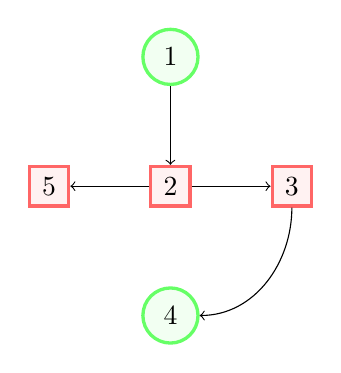
\begin{tikzpicture}[
            roundnode/.style={circle, draw=green!60, fill=green!5, very thick, minimum size=7mm},
            squarednode/.style={rectangle, draw=red!60, fill=red!5, very thick, minimum size=5mm},
        ]
        %Nodes
        \node[squarednode]      (maintopic)                              {2};
        \node[roundnode]        (uppercircle)       [above=of maintopic] {1};
        \node[squarednode]      (rightsquare)       [right=of maintopic] {3};
        \node[roundnode]        (lowercircle)       [below=of maintopic] {4};
        \node[squarednode]      (leftsquare)        [left=of maintopic]  {5};

        %Lines
        \draw[->] (uppercircle.south) -- (maintopic.north);
        \draw[->] (maintopic.east) -- (rightsquare.west);
        \draw[->] (rightsquare.south) .. controls +(down:7mm) and +(right:7mm) .. (lowercircle.east);
        \draw[->] (maintopic.west) -- (leftsquare.east);
    \end{tikzpicture}
\end{center}

\newpage

\begin{center}
    
\begin{tikzpicture}[transform canvas={scale=4.0}]
        \draw[blue] (0, 1) arc (90:-90:0.5cm and 1cm);
        \draw[dashed, red] (0, 1) arc (90:270:0.5cm and 1cm);
        \draw (0, 0) circle(1cm);
        \filldraw[red] (0, 1) circle (0.05);
        \filldraw[red] (0, -1) circle (0.05);
        \shade[ball color=blue!10!white,opacity=0.20] (0, 0) circle(1cm);
    \end{tikzpicture}
\end{center}

\newpage

\end{document}
